%TEX root = ../dissertation.tex

\chapter{Implementation}
\label{chapter:Implementation}

In this chapter, the first section \ref{Previous_architecture} will be about the previous control architecture, divided in subsections describing the previous open loop control scheme and describing the one developed at the same time by another student based on \gls{PBVS}. The second section \ref{developed_solution} is about the  design and implementation of the developed solutions, it will be divided in four subsections, the first one is about describing the approach, the second one is about the hardware and software tools used for this work, the third one is about the implementation of the first solution and fourth one is about the final implementation.

\section{Previous architecture}
\label{Previous_architecture}
\subsection{Open-loop}
The implemented system used before I began my work was an open loop control scheme (figure:\ref{pict:open_loop}). Once the trajectory is planned, execution module does not considering possibility of goal object movement or unexpected obstacles. In this approach robot is “blindfolded” what gives several drawbacks specially accuracy and reliability since the system does not have feedback on the control.
\begin{figure} [!ht]
    \centering
    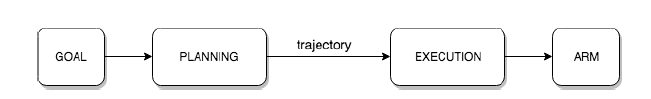
\includegraphics[width=0.75\linewidth]{images/open_loop.png}
    \caption{Open loop architecture}
    \label{pict:open_loop}
\end{figure}

Trajectory is planned, from the current pose to the desired pose, before the manipulator starts its motion. Execution is realized by a trajectory controller from Moveit! framework. The following module takes computed trajectory, which is a sequence of joints angles, converts them into the drivers speed and sends information to the servos of manipulator. 

\subsection{PBVS}

During the period of my internship, another student was working at the time, on the development on a new controller for the arm. This work was based on developing an optimization based Cartesian controller for the arm (from an input desired pose and the current position of the end effector computing joint velocities to reach the desired pose with constraints on joint position). Combining this work with a pose estimation algorithm developed by another student using also YOLO, a \gls{PBVS} is implemented (\ref{chap:pbvs}). It is using the head camera of the robot, so an EYE-TO-HAND configuration (figure:\ref{pict:eye_in_hand}).
\begin{figure} [!ht]
    \centering
    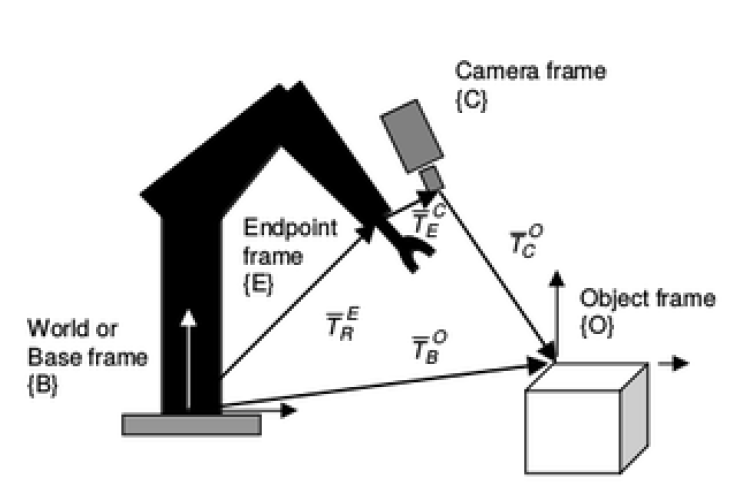
\includegraphics[width=0.95\linewidth]{images/pbvs.png}
    \caption{PBVS architecture developed by another student}
    \label{pict:pbvs_emilia}
\end{figure}

This controller is combining motion of the base and the arm. It has been designed as an optimization problem. For now, it applied constraints to avoid joint limits.

\section{Developed solutions}
\label{developed_solution}

\subsection{Approach}
Applying an Image Based Visual Servoing control law to Mbot 7DoF with an EYE-IN-HAND configuration is the subject of this work. This title is describing the working approach. The approach here is to use an \gls{IBVS} (\ref{chap:ibvs}). This control law is applied to a robotic manipulator that has 7 joints and 7\gls{DoF}. The camera is fixed on the end effector that is defined as an EYE-IN-HAND configuration (figure: \ref{pict:eye_in_hand}).
\subsubsection{Constraints}
The constraints for this work are:
\begin{itemize}
    \item Using an IBVS control law with an EYE-IN-HAND configuration
    \item No predefined object, the algorithm as to be as generic as possible
    \item The algorithm has to as close as real time as possible
    \item The working environment is not fixed, it is dynamic, the control law has to adapt to new environment and if the object move during the grasping approach
    \item Having a grasping approach, not only going to a certain pose but also think about grasping
\end{itemize}
\subsubsection{Why using an IBVS}
The two major benefits of using an \gls{IBVS} in a grasping approach are:
\begin{itemize}
    \item Avoiding calibration issues, the precision for grasping is really important, because a small error (cm) can lead to a grasping fail.
    \item Closed loop and able to be use in a dynamic environment
\end{itemize}
In the next subsection, the tools used for this work will be described hardware and software.

\subsection{Hardware and Software}
To achieved the design and implementation of the previously described approach, we did not start from scratch. We used existing libraries, software and also of course an already very advanced robot  hardware speaking robot, Mbot.
\subsubsection{Software}
\begin{itemize}
    \item 
\gls{ROS} is a middleware (\ref{pict:ros}). It is a computer software that provide services to software applications. It makes easier for software developers to implement communication and input/output, so they can focus on the specific purpose of their application.
\gls{ROS} is a flexible framework helping developers creates software for robots \cite{288}. It provides device drivers, collection of tools and libraries, visualizers, message-passing, package management, and more to simplify the task of creating complex applications across various robotics platforms. ROS is licensed under an open source. Developed controller is implemented in the Robot Operating System environment for the needs of integration the module with the team code base.
\begin{figure} [!ht]
    \centering
    
\includegraphics[width=0.35\linewidth]{images/ros.png}
    \caption{Robot Operating System, since 2007.}
    \label{pict:ros}
\end{figure}
    \item
\gls{ViSP} is a modular C++ library that allows fast development of visual servoing applications \cite{articlevisp}. ViSP is developed and maintained by the Inria Rainbow team located at Inria Rennes. The platform takes the form of a library which is divided in several modules (core, io, gui, vision, …). ViSP software environment features independence with respect to the hardware, simplicity, extendibility, and portability. ViSP also features a large library of elementary tasks with various visual features that can be combined together, an image processing library that allows the tracking of visual cues at video rate, a simulator, an interface with various classical frame grabbers, a virtual 6DoF robot that allows the simulation of visual servoing experiments, etc. The platform is implemented in C++ under Linux.

To use ViSP inside a ROS environment, ViSP ROS package was used. It also have been developed by Inria Rennes. It is an extension of the ViSP library. While ViSP is independent from ROS, in $visp_ros$ we benefit from ROS features.
\begin{figure} [!h]
    \begin{minipage}[b]{0.5\linewidth}
        \begin{center}
            
\includegraphics[width=0.8\linewidth]{images/bandeauViSP.png}
        \end{center}
        \label{pict:visp_logo}
    \end{minipage}
    \begin{minipage}[b]{0.5\linewidth}
      \begin{center}
        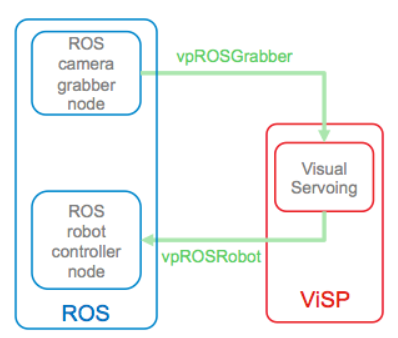
\includegraphics[width=0.6\textwidth]{images/visp_ros.png}
      \end{center}
    \end{minipage}
    \caption  {ViSP, Visual Servoing Platform, developed by Inria Rennes, 2005}
\end{figure}
    \item 
Gazebo is a simulation software that is highly compatible with ROS development. Robot simulation is an essential tool in every roboticist's toolbox. A well-designed simulator makes it possible to rapidly test algorithms, design robots, perform regression testing, and train AI system using realistic scenarios. Gazebo offers the ability to accurately and efficiently simulate populations of robots in complex indoor and outdoor environments.Gazebo is an open source software, improved by the community.
\begin{figure} [!h]
    \begin{minipage}[b]{0.4\linewidth}
        \centering
        
\includegraphics[width=1\textwidth]{images/gazebo.jpg}
    \end{minipage}
    \begin{minipage}[b]{0.6\linewidth}
      \begin{center}
        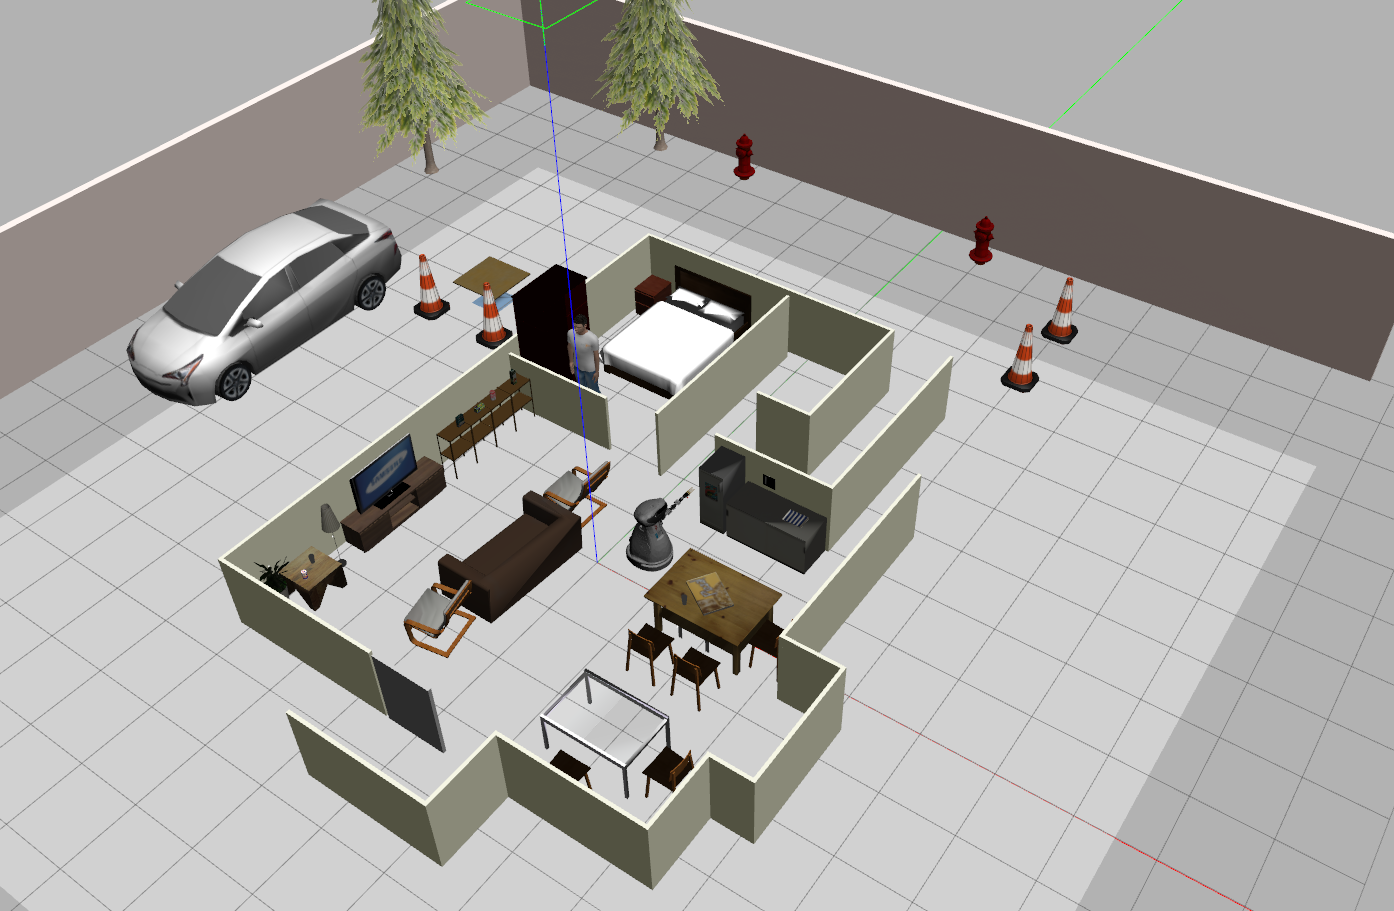
\includegraphics[width=0.8\textwidth]{images/gazebo_isr_testbeld.png}
      \end{center}
    \end{minipage}
    \caption{Gazebo, ROS friendly simulation software(left), ISR testbeld used to test robot tasks in Gazebo (right)}
\end{figure}
    \item 
\gls{URDF} is a package of a number of XML format files, used in \gls{ROS} to describe all elements of the robot. XML files contain specification of sensors, robot models, scenes and more. Each file of XML format has a corresponding in one or more programming language parser. In our project the URDF files contains the most essential information for this work about manipulator (number of joints, links lengths, joints limits, etc.) as well as information about the robotic base. It is also used to construct the robot model in Gazebo for example and in Rviz.
    \item 
\gls{YOLO} is a convolutional neural network used in this work to detect and extract features. It has been described in the the chapter \ref{chapter:Background} in section \ref{Object_detection}.
    \item 
Controlling arm servos (sending commands to the joints of the arm), to this purpose two possibilities:
    \begin{enumerate}
        \item  An inverse kinematic controller, that take as input a desired velocity vector of the end effector and compute the corresponding joint velocities to achieve the desired velocity for the end effector. This "controller" only controls the arm and not the arm and the base of the robot combined to be able to reach a larger area when having a grasping approach. The well known problem when using inverse kinematic as described in section \ref{chap:inversekinematics} is singularities and local minima.
        \item An optimization forward kinematic controller, developed during the time of my internship to use with his work on \gls{PBVS}. This "controller" controls the arm and the base at the same time. It takes as input a pose in world frame and output the joint velocities, more information on the section \ref{Previous_architecture}. Since it is an early development many problems appeared using this controller, like when doing the optimization not using the last joint or not taking as input velocities. One of my work was to convert this controller to be able to end effector velocities as input.
    \end{enumerate}

\end{itemize}

\subsubsection{Hardware}
\begin{itemize}
    \item Manipulator description
The manipulator used by the robot is a Cyton Gamma 1500 (figure: ) produced by Robai company. It is a 7DoF manipulator with a 3D printed end effector. Joints of the manipulator are made of two types of DYNAMIXEL smart actuators: MX-28 and MX-64 (figure:).
As it’s written in the product documentation, humanoid robot arms with many degrees of freedom, can reach around obstacles and through gaps, reconfigure for strength, and manipulate objects with dexterous fluid motion. This manipulator has kinematic redundancy, that enables placement of a hand or tool at a position and orientation in an unlimited number of ways. Presented manipulator model is no longer commercially available.
\begin{figure} [!ht]
    \begin{minipage}[b]{0.5\linewidth}
        \centering
        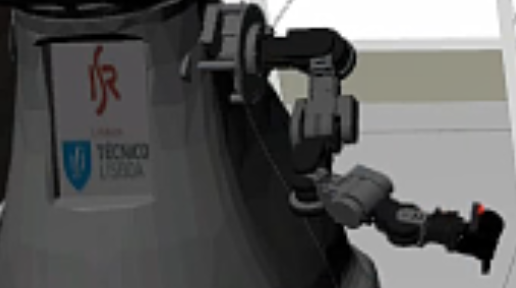
\includegraphics[width=0.8\textwidth]{images/manipulator_sim.png}
    \end{minipage}
    \begin{minipage}[b]{0.5\linewidth}
      \begin{center}
        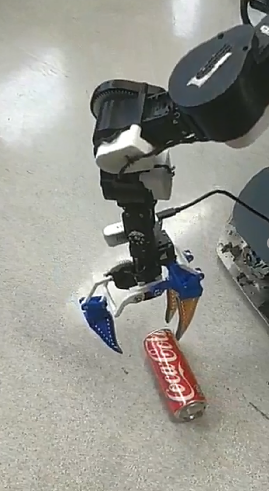
\includegraphics[width=0.35\textwidth]{images/real_robot_grasping_floor.png}
      \end{center}
    \end{minipage}
    \caption{Manipulator in simulation with Gazebo and defined by an \gls{URDF} file(left), Real manipulator fixed on Mbot (right)}
\end{figure}


\newpage
    \item 
The Intel® RealSense™ Depth Camera D435 uses stereo vision to calculate depth. It is USB-powered and consist of a pair of depth sensors, an RGB sensor, and an infrared projector. It is a close ranged depth camera that can read depth from about 0.17m to 0.8m. It is also really compact and light that makes this camera perfect for being fixed on the end effector.
\begin{figure} [!ht]
    \centering
    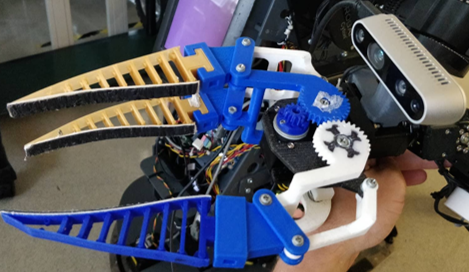
\includegraphics[width=0.5\linewidth]{images/camera_and_gripper_real.png}
    \caption{Camera and effector on Mbot}
    \label{pict:camera_gripper}
\end{figure}
\end{itemize}

In the next subsections we will present the developed solutions. The work will be divided in two part: a first solution and a final solution. When I start my internship, the robot was not equipped with the gripper camera fixed on the arm effector and before implementing your algorithm, it is usual to first test it inside simulation. So, the first implementation has been developed in simulation and the final solution has been implemented in simulation and inside the real robot. The main difference between these solutions is the way its initialized and the way the features are detected and extracted.

\subsection{1st solution}
  
The first solution is based on a simple feature detection and tracking method called blob detection and tracking. Blob detection methods aimed at detecting regions in an image that differ in properties such as color, brightness for example compared to surrounding regions. Informally, a blob is a region of an image in which some properties defined by the user are constant or approximately constant. In simulation this blob are black point a juice box.\\
The control scheme of this first implementation is described in the figure: \ref{pict:control_scheme_1}.
\begin{figure} [!ht]
    \centering
    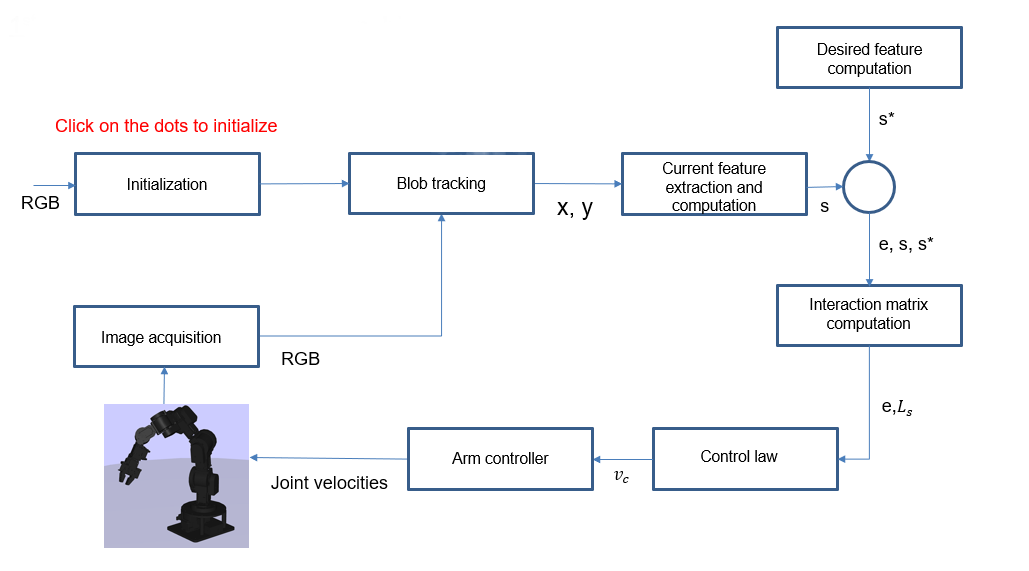
\includegraphics[width=1.\linewidth]{images/control_scheme_1.png}
    \caption{First implementation control scheme}
    \label{pict:control_scheme_1}
\end{figure}

The first step of this control scheme is the initialization, the user as to click with the mouse inside the display on the 4 dots. From this blob, the \gls{COG} is computed : one point with (x,y) coordinates. From



interaction matrix 2 parameters
scheme
pro cons

\subsection{Final solution}
interaction matrix 3 parameters
scheme
pro cons

\subsection{Results}

\subsubsection{1st implementation}


\subsubsection{Final implementation}



